\documentclass{article}
\usepackage[T1]{fontenc}
\usepackage{lmodern}
\usepackage{graphicx}
\usepackage{amsmath,amssymb}
\usepackage[a4paper,margin=2cm]{geometry}
\usepackage[absolute,overlay]{textpos}
\setlength{\TPHorizModule}{1mm}
\setlength{\TPVertModule}{1mm}
\usepackage[indonesian]{babel}
\usepackage{hyperref}
\setlength{\emergencystretch}{2em}
% unit: Halaman 80

\begin{document}

% === Halaman 80 (llm) ===

\vspace{264.33mm}

Tampilkan citra cover:\vspace{5mm}

Tampilkan citra stego:

% deskripsi: Citra cover yang menampilkan sekelompok mahasiswa di dalam kelas.
% bbox normalisasi: [0.0500, 0.0900, 0.4300, 0.9800]
\begin{textblock*}{79.80mm}(10.50mm,26.73mm)
\noindent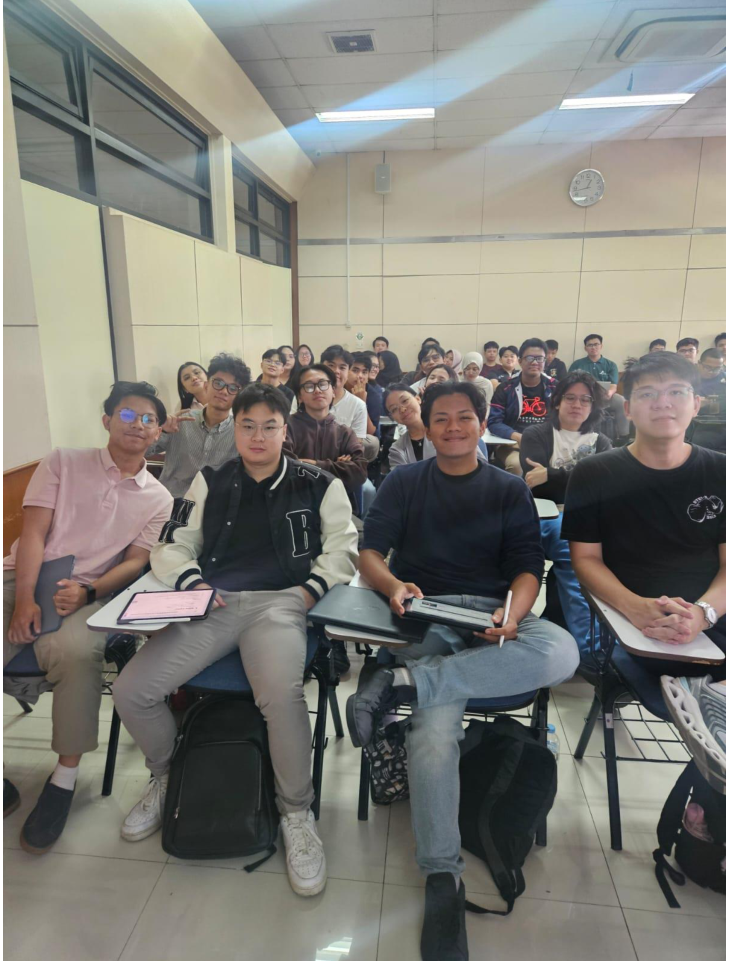
\includegraphics[width=79.80mm,height=264.33mm]{../../images/llm/page_080_img_01.png}%
\end{textblock*}

% deskripsi: Citra stego yang terlihat identik dengan citra cover, menampilkan sekelompok mahasiswa di dalam kelas.
% bbox normalisasi: [0.5000, 0.0900, 0.8800, 0.9800]
\begin{textblock*}{79.80mm}(105.00mm,26.73mm)
\noindent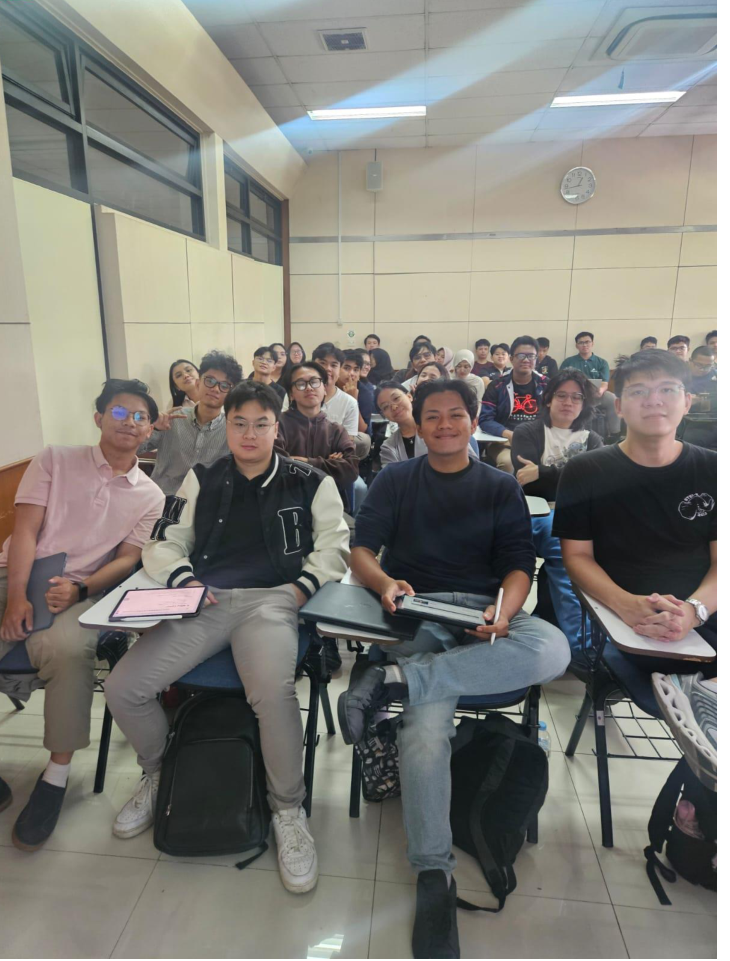
\includegraphics[width=79.80mm,height=264.33mm]{../../images/llm/page_080_img_02.png}%
\end{textblock*}

\end{document}
